\documentclass[12pt]{article}
\usepackage[letterpaper,top=2cm,bottom=2cm,left=2.7cm,right=2.7cm,marginparwidth=1.75cm]{geometry}
\usepackage{graphicx} % Required for inserting images
\usepackage[french]{babel}
\usepackage[T1]{fontenc}
\usepackage{listings}
\usepackage{float}
\usepackage{color}
\usepackage{xcolor}
\usepackage{tikzducks}
\usepackage{lipsum}
\usepackage{amsmath,amsthm}
\usepackage{amssymb}
\usepackage{changepage}
\usepackage{algorithm}
\usepackage{algpseudocode}
\usepackage{multicol} % Pour les colonnes
\usepackage[hidelinks]{hyperref}
\usepackage{csquotes}
\definecolor{dkgreen}{rgb}{0,0.6,0}
\definecolor{gray}{rgb}{0.5,0.5,0.5}
\definecolor{mauve}{rgb}{0.58,0,0.82}
\lstset{frame=tb,
  language=Python,
  extendedchars,  % Extended ASCII
  aboveskip=3mm,
  belowskip=3mm,
  showstringspaces=false,
  columns=flexible,
  basicstyle={\small\ttfamily},
  numbers=none,
  numberstyle=\tiny\color{gray},
  keywordstyle=\color{blue},
  commentstyle=\color{teal},
  stringstyle=\color{violet},
  breaklines=true,
  breakatwhitespace=true,
  tabsize=3
}
\usepackage{tikz}
\usetikzlibrary{shapes.geometric, arrows}
\tikzstyle{box} = [rectangle, 
minimum width=2cm, 
minimum height=1cm,
text centered, 
draw=black]
\tikzstyle{arrow} = [thick,->,>=stealth]
\usepackage[
backend=biber,
style=alphabetic,
sorting=ynt
]{biblatex}
\addbibresource{bib.bib}


\newcommand{\K}{\mathbb{K}}
\newcommand{\N}{\mathbb{N}}
\newcommand{\C}{\mathbb{C}}
\newcommand{\R}{\mathbb{R}}
\newcommand{\Rd}{\mathbb{R}^d}
\newcommand{\I}{\mathbf{I}}
\newcommand{\dcrochetg}{[\![}
\newcommand{\dcrochetd}{]\!]}
\newcommand\independent{\protect\mathpalette{\protect\independenT}{\perp}}
\def\independenT#1#2{\mathrel{\rlap{$#1#2$}\mkern2mu{#1#2}}}

%Gary's stuff 
\newtheorem{thm1}{Théorème}[section]
\newtheorem{lemme1}[thm1]{Lemme}
\newtheorem{prop1}[thm1]{Proposition}
\newtheorem*{rmq1}{Remarque}
\newtheorem*{exemple1}{Exemple}
\newtheorem*{defin1}{Définition}
%End of Gary's stuff


\begin{document}
\title{Rapport de projet tutoré : Étude de la chute des météorites sur Terre}
\author{Yannis Petit, Rassem Djimadoum, Duc-Khoi Nguyen \& Garance Malnoë \\ encadré.e.s par Jean-François Coeurjolly}
\date{Janvier-Avril 2025 - M1 SSD}

\pagenumbering{gobble}
\maketitle
\tableofcontents
\clearpage
\pagenumbering{arabic}
\section{Introduction}
Ce rapport présente le projet tutoré réalisé de janvier à avril 2025 dans le cadre de notre première année de Master en Statistique et Sciences des Données, sous la direction de Jean-François Coeurjolly. Ce projet se concentre sur l'analyse du jeu de données \textit{Meteorite Landings}, qui recense les météorites tombées au sol. Ce jeu de données est mis à disposition par la Meteoritical Society et est accessible sur l'Open Data de la NASA \cite{OpenData_NASA}.\\
\\
Au départ, ce projet n'a pas d'objectif défini ; l'idée initiale consiste à explorer librement le jeu de données et à identifier les axes d'analyse les plus pertinents. Cependant, Jean-François Coeurjolly nous a suggéré plusieurs pistes lors de notre premier échange :\\
\begin{itemize}
	\item[-] Étudier la dimension temporelle des données, notamment la présence d'une saisonnalité ou d'une tendance.\\
	\item[-] Analyser les relations entre différentes variables du jeu de données, en particulier l'influence de la masse des météorites.\\
	\item[-] Construire un modèle prédictif du nombre de météorites tombées dans un pays en fonction de sa superficie et de sa localisation géographique.\\
	\item[-] Réaliser une étude spatiale pour déterminer si certaines régions sont plus touchées et, le cas échéant, identifier les sources des différences.\\
	\item[-] Visualiser les chutes de météorites sur un planisphère.\\
\end{itemize}
Cependant, en raison de la nature des données, nous n'explorons finalement pas toutes ces pistes. Néanmoins, nous dégageons de nouvelles perspectives que nous détaillons par la suite.\\
\\
Nous débutons ce rapport par une présentation de notre organisation de travail ainsi que des outils, langages et bibliothèques utilisés. Nous poursuivons avec une analyse exploratoire des données, comprenant des analyses univariées et multivariées, qui nous amènent à discuter des pistes à explorer. Ensuite, nous étudions la modélisation des chutes de météorites à l'aide des processus ponctuels, avant de proposer une visualisation interactive du jeu de données sur un globe. Enfin, nous concluons par une réflexion sur l'impact environnemental du projet.\\
\newpage

\section{Organisation, Outils, bibliothèques \texttt{R} et \texttt{Python}}
Notre projet a débuté en janvier, contrairement aux autres groupes qui ont commencé en octobre. Ce décalage est dû au fait que nous ayons initialement commencé à travailler sur  premier projet d'application Shiny pour le Conseil National des Universités, qui n'a finalement pas abouti. Suite à cela, notre tuteur nous a proposé de nous engager dans ce nouveau projet.\\
\\
Pour assurer un suivi régulier de notre avancement, nous avons organisé six réunions d'environ 45 minutes, toutes les deux semaines, avec notre encadrant. Ces rencontres nous ont permis de faire le point sur nos progrès, de poser nos questions et d'ajuster notre travail en fonction des retours reçus.\\
\\
En ce qui concerne la répartition du travail, chaque membre de l'équipe a contribué de manière spécifique. Garance a pris en charge l'exploration des données et a également collaboré avec Rassem sur la modélisation par les processus ponctuels, où elle s'est concentrée sur la partie mathématique tandis que Rassem s'est occupé de la simulation. Yannis et Duc-Khoi ont chacun travaillé sur la visualisation en 3D, Duc-Khoi utilisant \texttt{Python} pour sa partie, tandis que Yannis s'est concentré sur \texttt{R}. Pour la rédaction du rapport, chaque membre a rédigé la section correspondant à sa contribution. Garance a également pris en charge l'introduction et la partie organisation, tandis que Rassem a rédigé la section sur l'impact environnemental et Yannis s'est occupé de la conclusion.\\
\\
Nous n'avons pas mis en place d'outils d'organisation formels, tels qu'un diagramme prévisionnel ou d'autres outils présentés lors de nos cours de gestion de projet que nous avions alors mis en oeuvre pour notre projet inital. Nous avons privilégié des discussions formelles et informelles pour définir les tâches à accomplir et faire le point avant chaque rendez-vous avec notre encadrant, chacun travaillant de manière autonome sur sa partie.\\
\\
Concernant les langages de programmation, nous avons opté pour un mélange de \texttt{R} et de \texttt{Python} afin de tirer parti des avantages offerts par les deux langages. Pour l'exploration des données, nous avons utilisé \texttt{Python} en raison de ses bibliothèques intéressantes pour la création de graphiques interactifs, telles que \texttt{Plotly} et \texttt{Shapely}. En revanche, nous avons choisi R pour produire des graphiques esthétiques avec \texttt{ggplot2} et pour réaliser des tests d'analyse multivariée. Pour les processus ponctuels, \texttt{R} s'est avéré être le choix idéal grâce à la bibliothèque \texttt{Spatstat},  présentée dans le livre \textit{Spatial Point Patterns - Methodology and Applications with \texttt{R}} \cite{analysing_spacial_points} fourni par Jean-François Coeurjolly, qui était spécifiquement axé sur \texttt{R}. Pour la visualisation 3D, nous avons décidé de travailler à la fois sur \texttt{R} et \texttt{Python}, ce choix étant explicité dans la partie correspondante.\\
\\
Enfin, pour les outils de développement, nous avons hébergé notre code sur GitHub et utilisé Visual Studio Code (VSCode) ainsi que RStudio pour la rédaction de notre code selon les langages utilisés et les préférences de chacun.\\
\\
Packages \texttt{Python} : \texttt{geopandas}, \texttt{pandas},\texttt{matplotlib}, \texttt{numpy}, \texttt{plotly} et \texttt{shapely}.\\
Packages \texttt{R} : \texttt{corrr}, \texttt{dplyr}, \texttt{ggplot2}, \texttt{leaflet}, \texttt{patchwork},\texttt{rnaturalearth}, \texttt{scales}, \texttt{sf}, \texttt{shiny},\texttt{shinydashboard}, \texttt{shinyjs}, \texttt{spastat}, \texttt{threejs}, \texttt{xtable} et 
\texttt{patchwork}.
\newpage
\section{Exploration des données}
L'analyse exploratoire des données constitue la première étape de notre projet. Notre objectif est de comprendre la distribution de chacune des variables tout en identifiant les données manquantes susceptibles d'influencer nos possibilités d'étude par la suite. Au cours de cette exploration, nous nous penchons également sur les relations entre les variables à travers divers tests statistiques. Cette approche nous permet de déterminer les axes d'investigation que nous souhaitons approfondir par la suite dont nous discutons par la suite.\\
\\
Pour réaliser les analyses univariées, nous commençons par utiliser \texttt{Python} en tirant parti des bibliothèques \texttt{numpy}, \texttt{pandas}, \texttt{geopandas}, \texttt{plotly} et \texttt{shapely}, dont nous avons l'habitude et qui nous offrent la possibilité de créer des planisphères interactifs. Par la suite, nous réalisons également certaines analyses avec \texttt{R}, qui facilite la gestion des sorties graphiques grâce à \texttt{ggplot2}. En ce qui concerne les analyses multivariées, nous nous concentrons exclusivement sur \texttt{R}, qui propose directement de nombreux tests statistiques adaptés à nos besoins. Le code de ces analyses est structuré dans les fichiers \texttt{exploration.ipynb} pour la partie en \texttt{Python} et \texttt{script\_analyses\_multivariées.R} pour la partie en \texttt{R}. Tous ces fichiers sont accessibles sur le repository GitHub du projet, dans le dossier intitulé "Exploration des données".\\
\\
Le jeu de données est composé de 45716 entrées décrites par neuf variables :

{\setlength{\baselineskip}{1.5\baselineskip} % Set a larger baselineskip for the itemize environment
\begin{itemize}
\item[-] \textbf{name} (qualitative nominale): le nom de la météorite.
\item[-] \textbf{nametype} (qualitative binaire) : le type d'objet soit "Valid" soit "Relict", Relict signifiant qu'il s'agit d'un objet très déformé considéré comme probablement d'origine météorite.
\item[-] \textbf{recclass} (qualitative nominale) : la classe de la météorite (ex : L5, H6, L5, ...).
\item[-] \textbf{mass} (quantitative continue) : la masse de la météorite en grammes.
\item[-] \textbf{fall} (qualitative binaire) : la nature de l'observation soit si la chute de la météorite a été observée (fell) ou si elle a été trouvée au sol (found).
\item[-] \textbf{year} (quantitative continue) : l'année où la météorite a été recensée.
\item[-] \textbf{reclat} (quantitative continue) : latitude où la météorite a été trouvée.
\item[-] \textbf{reclong} (quantitative continue) : longitude où la météorite a été trouvée.
\item[-] \textbf{geoLocation} : le couple de la latitude et de la longitude.
\end{itemize}
} % End of the larger baselineskip scope

\subsection{Analyses univariées}
\subsubsection*{Name}
Il n'y a pas de données manquantes pour le nom des météorites et tous les noms sont uniques. Par curiosité, nous avons regardé la répartition du choix de la première lettre :
\begin{figure}[H]
\centering
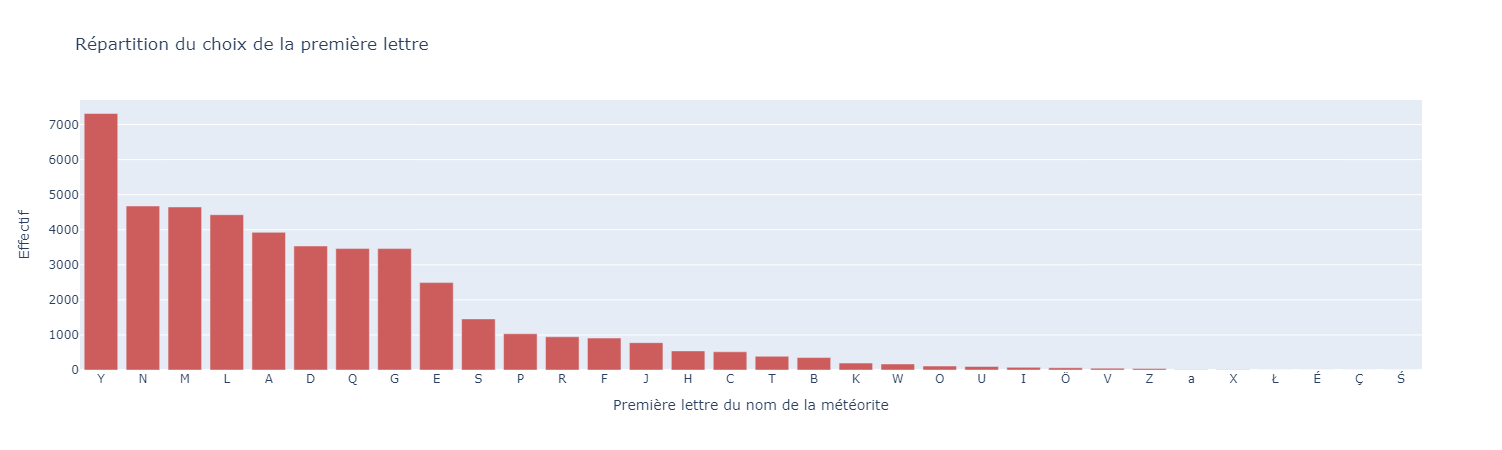
\includegraphics[width=16cm]{Images/exploration/name_barplot_lettres.png}
\caption{Diagramme en barres du choix de la première lettre du nom des météorites}
\end{figure}
Nous constatons que la lettre Y ressort nettement plus souvent que les autres. Cela n'est pas une coïncidence mais c'est lié aux conventions de nommage des météorites \cite{Convention_nommage_meteorites} : la grande majorité des météorites sont nommées d'après la localité géographique où elles ont été trouvées avec éventuellement une référence numérique après le nom si de nombreuses météorites sont collectées dans la zone. La popularité de la lettre Y est liée aux nombreuses expéditions japonaises effectuées sur le glacier Yamato en Antartique dont ces météorites tiennent leur nom. Sur les 7315 météorites dont le nom commence par la lettre Y, 7269 ont été répertoriées sur le glacier Yamato. De même pour la lettre N, sur 4667 météorites, 4499 météorites commencent par "Northwest Africa" suivi d'un numéro permettant d'identifier la météorite.
\subsubsection*{Nametype}
Cette variable n'a pas de données manquantes. Comme expliqué précédemment, c'est une variable qualitative binaire décrivant si la météorite a bien été identifiée comme valide (Valid) ou s'il s'agit d'un objet fortement déformé qui est probablement d'origine météorite (Relict). Une large majorité de entrées du jeu de données sont considérées comme valides : 45641 météorites valides soit 99,8\% contre 75 "Relict" soit 0,02\%.
\subsubsection*{Recclass}
Il n'y a pas de donnée manquante pour la variable \textbf{recclass} correspondant à la classification de la météorite. Le jeu de données compte 422 classes différentes mais les classes L5, L6, H5, H6, LL5 et LL6 sont nettement majoritaires et représentent près de 74\% du jeu de données comme nous pouvons le voir sur la figure ci-dessous :
\begin{figure}[H]
\centering
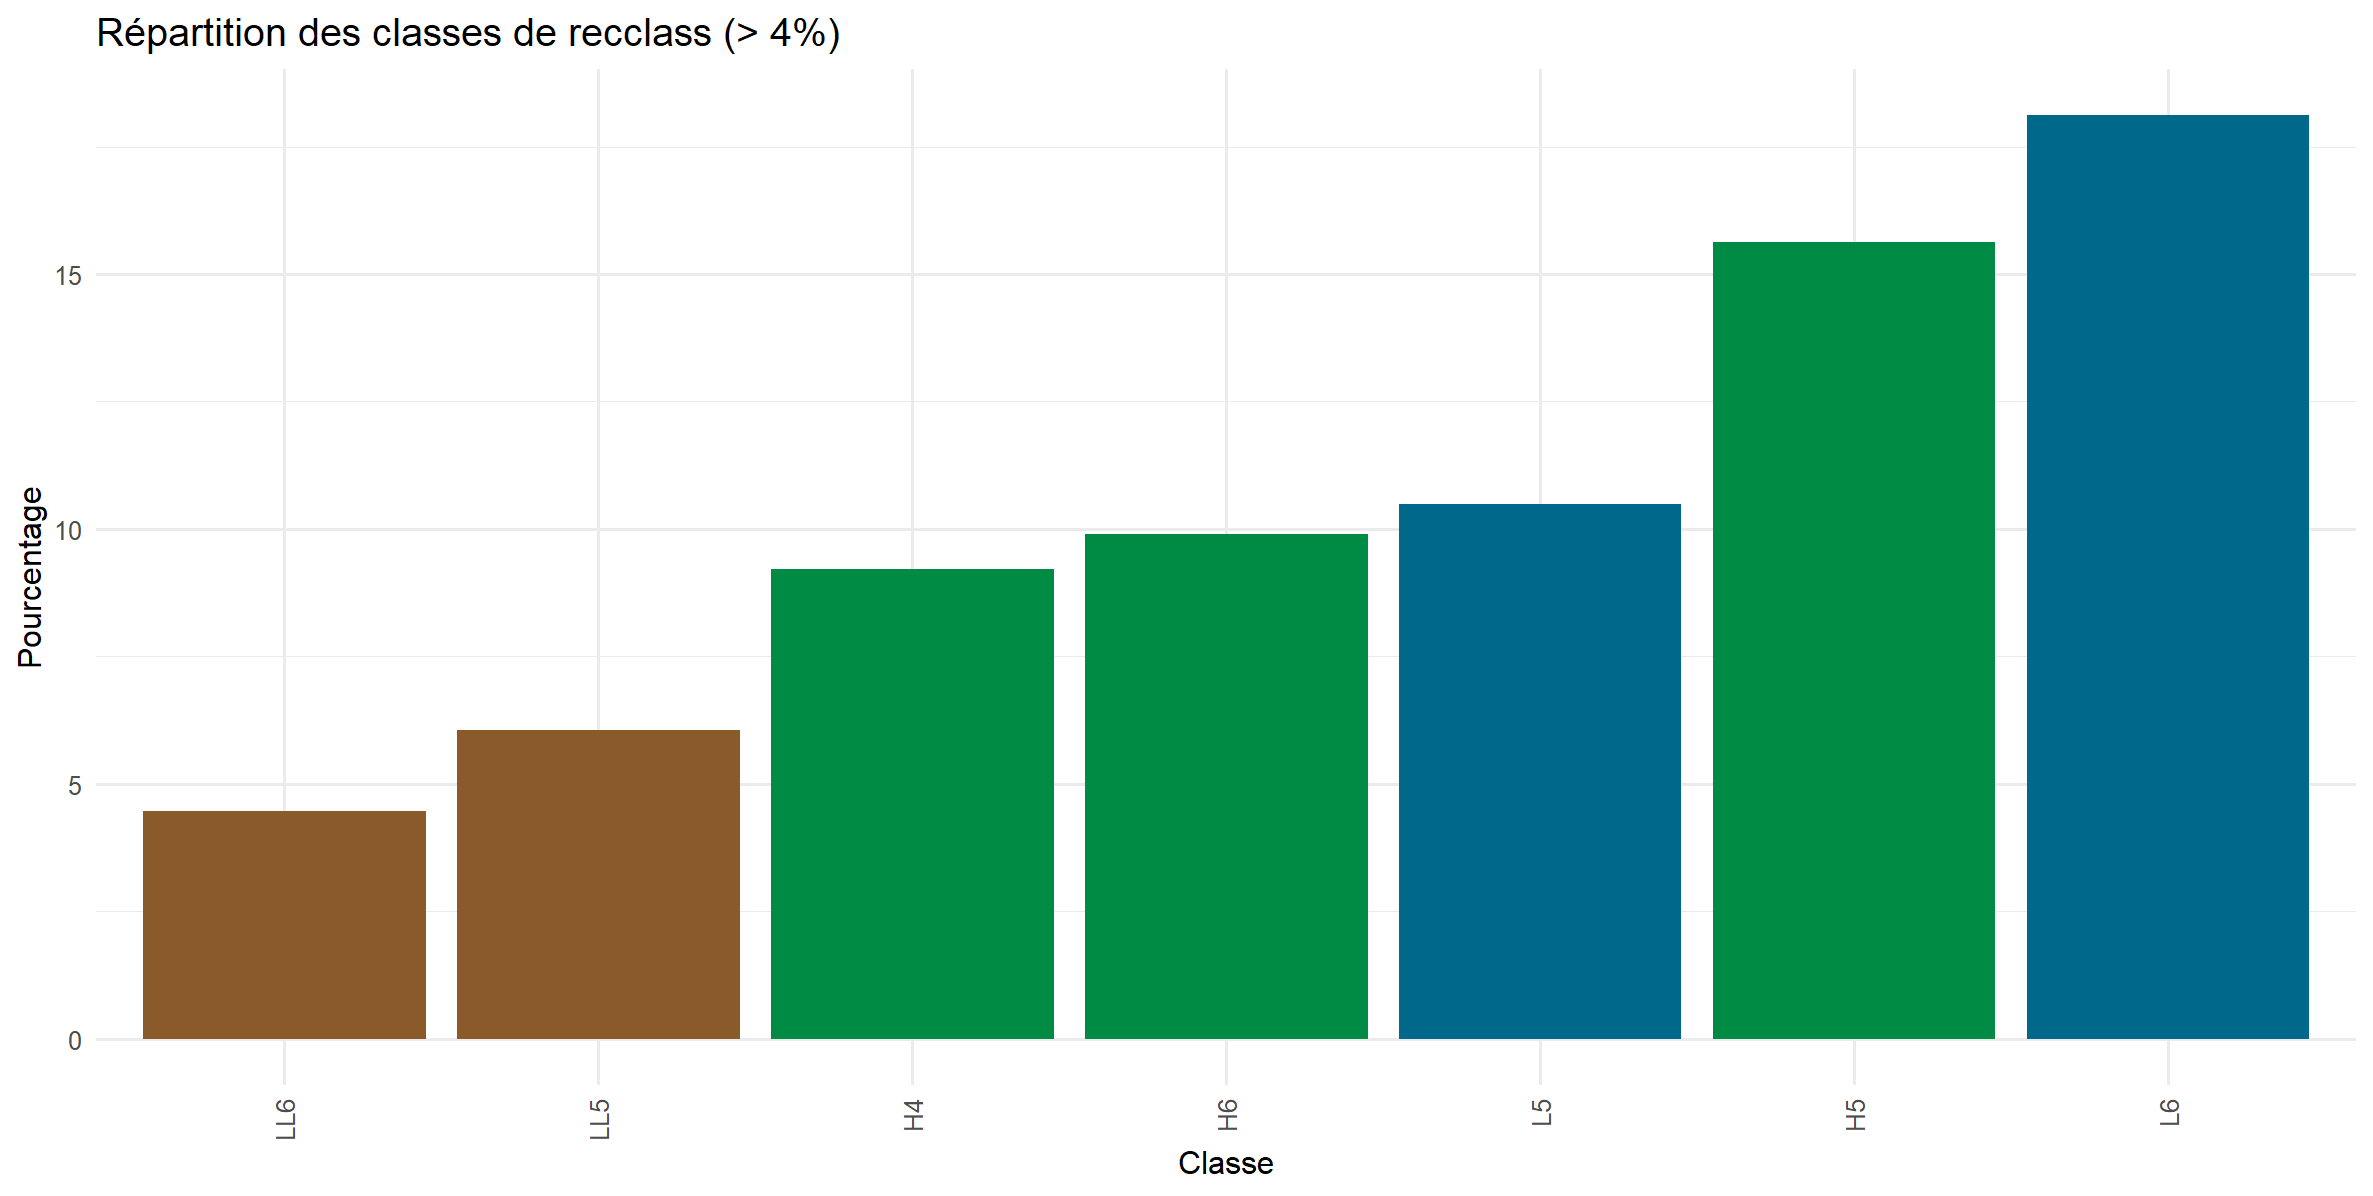
\includegraphics[width=17cm]{Images/exploration/recclass_piechart_class.png}
\caption{Piechart des classes de météorites}
\end{figure}
Ces 6 classes sont celles de chondrites ordinaires \cite{Classification_meteorites}. Les lettres L, H et LL correspondent aux trois sous-groupes des chrondrites ordinaires : H pour "High Iron" pour celles contenant 25-30\% de fer et de métal libre, L pour "Low Iron" pour celles contenant 20-25\% de fer et moins de métal libre et LL pour celles contenant encore moins de fer (environ 15-20\%) et très peu de métal libre. Le numéro qui suit correspond au degré de métamorphisme, compris entre 3 et 7, il indique le niveau des modifications subies par la météorite lors de sa chute dues à la pression et la chaleur modifiant sa composition minéralogique. Plus le numéro est élevé plus l'altération est importante.
\subsubsection*{Mass}
Il manque 131 données pour la variable \textbf{Mass} soit moins de 0,3\% du jeu de données. L'analyse de cette variable révèle tout d'abord une très grande hétérogénéité dans les valeurs possibles : plusieurs milliers de météorites pèsent moins de cinq grammes tandis que la plus grosse pèse 60 tonnes.\\
\\
\\
\begin{tikzpicture}

% Dessiner la boîte (boxplot) - proportions arbitraires
\draw[thick] (1, 0.25) rectangle (8, 1.75); % Boîte du boxplot

% Médiane (ligne à l'intérieur de la boîte)
\draw[thick] (4.5, 0.25) -- (4.5, 1.75); % Ligne médiane
\draw[thick] (10, 0.25) -- (10, 1.75);

% Moustaches (whiskers)
\draw[thick] (0, 0) -- (0, 2); % Moustache gauche

\draw[thick] (14.5, 0) -- (14.5, 2); % Moustache droite

%Lignes horizontales
\draw[thick] (0,1) -- (1,1);
\draw[thick] (8,1)--(9,1);
\draw[dashed] (9,1)--(14,1);
\draw[thick] (14,1)--(14.5,1);

% Ajouter des textes en dessous du boxplot
\node at (0, -0.5) {Min};
\node at (1,-0.5) {Q1};
\node at (4.5, -0.5) {Médiane};
\node at (8,-0.5) {Q3};
\node at (10, -0.5) {Moyenne};
\node at (14, -0.5) {Max};

\node at (0, -1) {0};
\node at (1,-1) {7,2g};
\node at (4.5, -1) {32,6g};
\node at (8,-1) {202,6g};
\node at (10, -1) {13,3kg};
\node at (14, -1) {60 tonnes};


\end{tikzpicture}
\\
\\
En fait, près de 75\% des météorites pèsent moins de 200 grammes mais la moyenne est à 13kg : la très large majorité des météorites recensées sont très légères mais le jeu de données recense quelques météorites très massives qui expliquent donc la moyenne très élevée. Dans les faits, seules 1388 météorites font plus de 10kg soit environ 3\% du jeu de données. Cela est lié au fait que, lors de leur chute, les météorites se vaporisent et se fragmentent sous l'effet de la pression et de la chaleur et au fait qu'elles puissent également se fragmenter lors de l'impact. De plus, en réalité, la proportion de (très) petites météorites est sûrement encore plus importante puisque les météorites les plus massives ont plus de chances d'être découvertes tandis que les petites météorites passent inapercues et peuvent être aisement confondues avec des roches terrestres empêchant ainsi leur recensement.
\subsubsection*{Fall}
Il n'y a pas de données manquantes pour cette variable. La très large majorité des météorites ont été trouvées (Found) et peu de météorites ont été obeservées lors de leur chûte (Fell), elles représentent seulement 2,5\% du jeu de données.
\subsubsection*{Year}
Pour cette variable, on compte 291 entrées manquantes ainsi qu'une donnée abérrante d'une météorite répertoriée comme tombée en 2101 que nous excluons de notre analyse. Comme pour la variable \textbf{Mass}, il y a de grandes disparités dans la distribution des valeurs :\\
\\
\begin{tikzpicture}

% Dessiner la boîte (boxplot) - proportions arbitraires
\draw[thick] (6, 0.25) rectangle (12, 1.75); % Boîte du boxplot

% Médiane (ligne à l'intérieur de la boîte)
\draw[thick] (9.5, 0.25) -- (9.5, 1.75); % Ligne médiane
\draw[thick] (7.2, 0.25) -- (7.2, 1.75); % Ligne moyenne

% Moustaches (whiskers)
\draw[thick] (0, 0) -- (0, 2); % Moustache gauche
\draw[thick] (14.5, 0) -- (14.5, 2); % Moustache droite

%Lignes horizontales
\draw[thick] (0,1) -- (1,1);
\draw[dashed] (1,1) -- (4,1);
\draw[thick] (4,1) -- (6,1);
\draw[thick] (12,1) -- (14.5,1);

% Ajouter des textes en dessous du boxplot
\node at (0, -0.5) {Min};
\node at (6,-0.5) {Q1};
\node at (7.2,-0.5) {Moyenne};
\node at (9.5, -0.5) {Médiane};
\node at (12,-0.5) {Q3};
\node at (14, -0.5) {Max};

\node at (0, -1) {860};
\node at (6,-1) {1987};
\node at (7.2,-1) {1991};
\node at (9.5, -1) {1998};
\node at (12,-1) {2003};
\node at (14, -1) {2013};


\end{tikzpicture}
\\
\\
Nous pouvons tout de suite voir que la grande majorité des valeurs sont très récentes : même si le jeu de données contient des météorites datant du IXème siècle, plus de 75\% des météorites recensées datent d'il y a moins de 50 ans. Cependant, cette variable nous permet de nous rendre compte que le jeu de données n'est pas récent ou pas mis à jour récemment puisque la dernière météorite recensée date de 2013 bien que d'autres météorites soient tombées sur Terre et aient été trouvées depuis. Intéressons-nous alors plus précisément aux 50 dernières années (1963-2013) :\\
\begin{figure}[H]
\centering
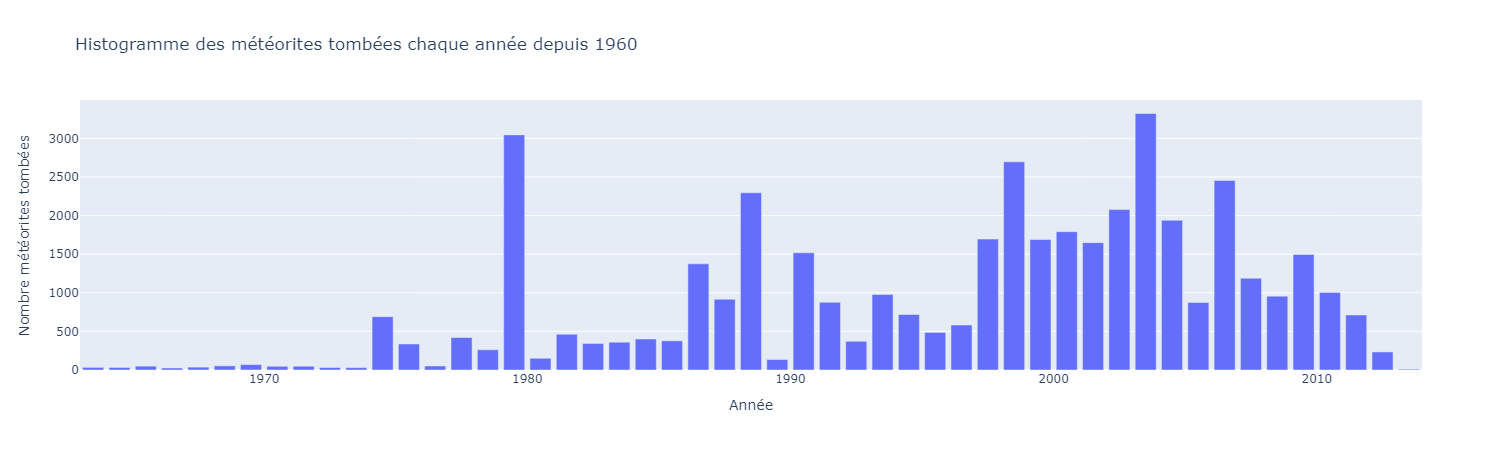
\includegraphics[width=16cm]{Images/exploration/histogramme1963-2013.png}
\caption{Répartition des météorites tombées entre 1963 et 2013}
\end{figure}
Nous observons une nette augmentation du nombre de météorites recensées à partir de 1974. Nous pouvons alors nous poser la question de la source de l'absence de données dans les années précédentes : est-ce que réellement peu de météorites sont tombées ou n'ont-elles juste pas été référencées ?\\
\\
Avant les années 1970, la détection de météorites reposait principalement sur des découvertes fortuites ou des témoignages. Les années 1970 ont vu l'essor des réseaux de surveillance qui ont permis un suivi plus rigoureux des météorites comme le Meteorite Observation and Recovery Projet \cite{Article_Canada_1970} lancé au Canada en 1974 ainsi que la mise en place de bases de données centralisées comme celle de la \textit{Meteoritical Society} \cite{BDD_centralisees} et de missions de recherche comme le programme \textit{The Antarctic Search for Meteorites} \cite{Mission_recherche_antartictique} lancé au milieu des années 1970. Ainsi, l'hypothèse que les météorites n'étaient pas correctement recensées avant les années 1970 semble assez cohérente.

\subsubsection*{Location}
Nous regroupons l'étude des variables \textbf{reclat}, \textbf{reclong} et \textbf{geolocation} dans l'étude de la variable \textbf{location} regroupant l'information de la latitude et de la longitude.\\
\\
Cette variable est celle avec le plus de données manquantes : 7315 entrées ne présentant pas à chaque fois la donnée de longitude, de latitude et de geolocation, soit environ 16\% du jeu de données. Dans un premier temps, nous pouvons visualiser sur le planisphère où sont tombées les météorites répertoriées :\\
\begin{figure}[H]
\centering
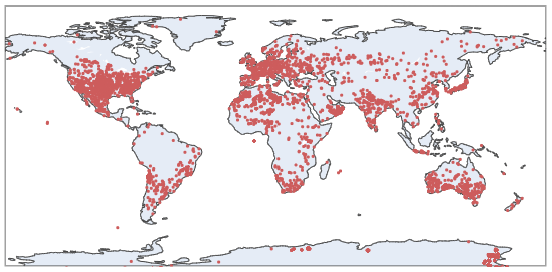
\includegraphics[width=14cm]{Images/exploration/points_monde.png}
\caption{Emplacement des chutes des météorites}
\end{figure}
Nous pouvons observer que certaines régions, comme les États-Unis, l’Europe de l’Ouest, le Japon, l’Afrique du Nord et le sud de l’Australie, concentrent une grande partie des recensements. À l’inverse, d’autres zones, telles que le nord du Canada, la Russie ou la forêt amazonienne, sont presque dépourvues de données. Sans surprise, les zones maritimes sont totalement absentes de notre jeu de données, puisqu’il ne répertorie que les météorites tombées sur des terres émergées.\\
\\
Cette répartition inégale met en évidence un biais de recensement important : les régions à faible densité de population, comme la forêt amazonienne ou les territoires du nord du Canada, comptent peu ou pas d’observations, contrairement aux zones fortement peuplées, comme l’Europe de l’Ouest, où les découvertes sont bien plus fréquentes. La seule exception notable à cette tendance est l’Antarctique, où de nombreux recensements ont été réalisés. Mais cette spécificité s’explique par les nombreuses missions de recherche dédiées à l’étude des météorites dans cette région \cite{Mission_recherche_antartictique}. En effet, les déserts glacés de l’Antarctique représentent des conditions idéales pour l’identification des météorites, facilitant leur repérage et leur collecte.\\
\\
Nous pouvons compléter cette première étude par une étude séparée de la latitude et de la longitude :\\
\\
\begin{figure}[H]
\centering
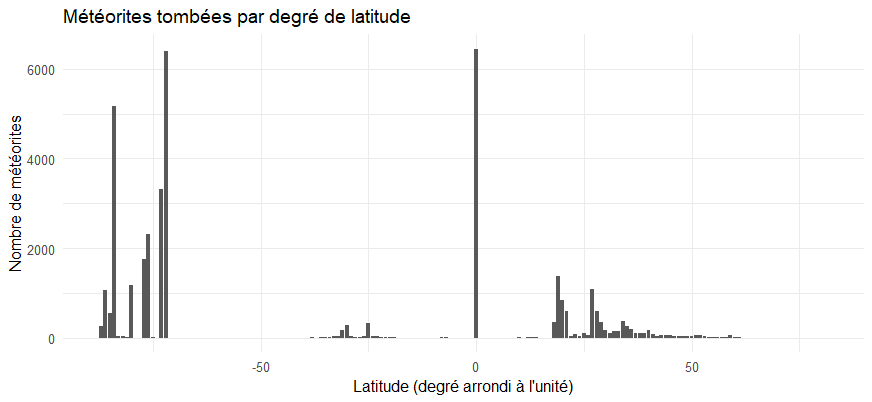
\includegraphics[width=16cm,height=6cm]{Images/exploration/histogramme_latitude.png}
\caption{Latitude des météorites}
\end{figure}
\begin{figure}[H]
\centering
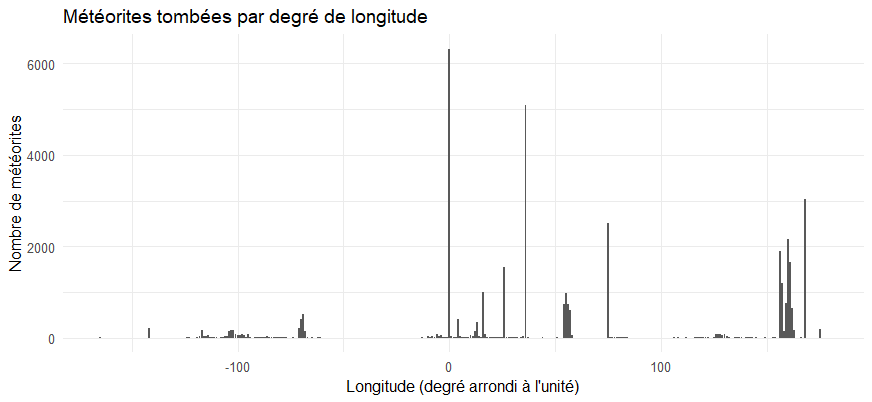
\includegraphics[width=16cm,height=6cm]{Images/exploration/histogramme_longitude.png}
\caption{Longitude des météorites}
\end{figure}

L'histogramme des latitudes montre une distribution inégale avec plusieurs tendances marquées. On observe un nombre particulièrement élevé d'impacts aux latitudes inférieures à -70°, correspondant aux nombreux points recensés en Antarctique. En revanche, la répartition est plus diffuse entre 15° et 60° Nord, couvrant des régions comme l'Europe de l'Ouest et l'Amérique du Nord. Un autre pic notable apparaît pour la latitude 0° précisément, cependant, sur la carte précédente on observe assez peu de données sur cette latitude, cette anomalie est en réalité due au fait que certains points aient été renseignés aux coordonnées (0,0) lorsque les coordonnées exactes n'ont pas pu être récupérées malgré le fait que certaines de ces météorites proviennent d'Antarctique comme, par exemple, 1666 observations provenant du glacier Yamato.  Il est difficile de dire précisément combien des 6214  observations aux coordonées (0,0) sont faussement renseignées mais nous pensons qu'elles forment probablement une grande part.\\
\\
L'analyse des longitudes révèle également une répartition très hétérogène. On retrouve le pic en 0 lié aux données faussement renseignées en (0,0) mais correspondant également  à l'Europe de l'Ouest et au nord de l'Afrique. D'autres concentrations apparaissent entre -150° et -162°, suggérant une fréquence plus élevée d'impacts en Australie et en Antarctique.\\
\\
Nous analysons ensuite la répartition du nombre de météorites par pays à l'aide des contours des pays proposé par le projet \textit{Natural Earth} \cite{Natural_Earth} :
\begin{figure}[H]
 \centering 
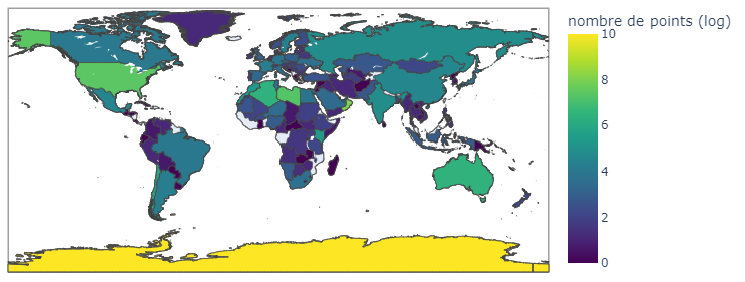
\includegraphics[width=17cm]{Images/exploration/map_points_countries_avec_echelle.png}
 \caption{Nombre de météorites recensées par pays}
 \end{figure}
Sans surprise, l’Antarctique est le territoire où le plus grand nombre de météorites a été recensé, suivi notamment des États-Unis, de la Libye, d’Oman, de l’Australie et de l’Algérie qui correspondent bien aux régions identifiées précédemment. Cependant, cette première visualisation ne prend pas en compte la taille des pays qui varie considérablement (par exemple, 7 700 000 km² pour l’Australie contre 309 000 km² pour l'Oman), ce qui peut biaiser l’interprétation des résultats. Afin de mieux appréhender cette distribution, nous calculons le nombre de météorites rapporté à la superficie du pays en km² :
\begin{figure}[H] 
\centering
 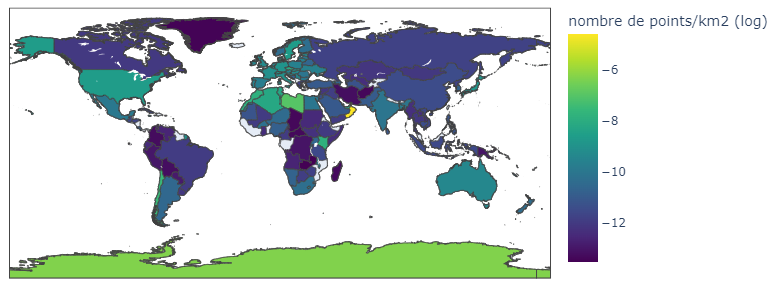
\includegraphics[width=17cm]{Images/exploration/map_points_km2_avec_echelle.png}
 \caption{Densité de météorites recensées par km² et par pays}
 \end{figure}
Cette nouvelle représentation met en évidence plusieurs tendances intéressantes : Oman ressort davantage que dans la carte précédente, tandis que l’Australie et l’Antarctique, bien qu’ayant un grand nombre de météorites recensées, apparaissent moins dominantes lorsque nous tenons compte de leur superficie. Par ailleurs, les pays d’Europe de l’Ouest présentent des valeurs comparables à celles des États-Unis et des pays d’Afrique du Nord-Ouest.\\
\\
Enfin, nous avons également regardé la répartition des météorites dans le monde selon la masse, mais aucune tendance n'est ressortie.

\subsection{Analyses multivariées}
Nous poursuivons notre analyse du jeu de données par des analyses multivariées par le biais de tests sur les croisements des différentes variables entre elles.
\subsubsection*{Analyse qualitative-qualitative}

Pour le croisement de variables qualitatives entre elles, nous effectuons des tests de $\chi^2$. Pour chaque croisement, nous donnons dans le tableau suivant la p-value associée au résultat du test.
\begin{table}[H]
\centering
\begin{tabular}{rlr}
  \hline
 & Variables & p\_value \\ 
  \hline
1 & nametype - recclass & < $2\times 10^{-16}$  \\ 
  2 & nametype - fall & 0.9085 \\ 
  3 & recclass - fall & < $2\times 10^{-16}$  \\ 
   \hline
\end{tabular}
\caption{Résultats des tests de $\chi^2$}
\end{table}
\subsubsection*{Analyse quantitative-quantitative}
Pour le croisement de variables quantitatives entre elles, nous regardons cette fois le coefficient de corrélation de Pearson. Les résultats sont résumés dans le tableau ci-contre :
\begin{table}[H]
\centering
\begin{tabular}{rlrrrr}
  \hline
 & term & mass..g. & year & reclat & reclong \\ 
  \hline
1 & mass..g. &  & -0.1219 & 0.0292 & -0.0219 \\ 
  2 & year & -0.1219 &  & -0.1050 & 0.0903 \\ 
  3 & reclat & 0.0292 & -0.1050 &  & -0.5932 \\ 
  4 & reclong & -0.0219 & 0.0903 & -0.5932 &  \\ 
   \hline
\end{tabular}
\caption{Corrélations de Pearson}
\end{table}
A priori, aucune des variables ne sont très corrélées, la plus forte corrélation est entre la latitude et la longitude à $-0.59$ qui reste relativement faible et peut s'expliquer par le biais de recensement identifié lors des analyses univariées.

\subsubsection*{Analyse quantitative-qualitative}
Avant de faire les croisements entre variables quantitatives et qualitatives, nous testons l'hypothèse de normalité des données avec un test de Shapiro-Wilk. Pour l'ensemble des variables, le test ressort toujours comme étant très significatif (p-valeur < $2\times 10^{-16}$), nous ne considérons donc pas les données comme respectant l'hypothèse de normalité. Nous effectuons donc un test de Kruskal-Wallis ou de Mann-Whitney pour tester le lien entre deux variables, ces deux tests étant  robustes à l'absence de normalité.
\begin{table}[H]
\centering
\begin{tabular}{rllr}
  \hline
 & Variable quantitative & Variable qualitative & p-value \\ 
  \hline
1 & mass..g. & nametype & < $2\times 10^{-16}$ \\ 
  2 & year & nametype &< $2\times 10^{-16}$  \\ 
  3 & reclat & nametype &< $2\times 10^{-16}$ \\ 
  4 & reclong & nametype & 0.1026 \\ 
  5 & mass..g. & recclass & < $2\times 10^{-16}$  \\ 
  6 & year & recclass & < $2\times 10^{-16}$  \\ 
  7 & reclat & recclass & < $2\times 10^{-16}$  \\ 
  8 & reclong & recclass & < $2\times 10^{-16}$  \\ 
  9 & mass..g. & fall &< $2\times 10^{-16}$  \\ 
  10 & year & fall & < $2\times 10^{-16}$  \\ 
  11 & reclat & fall &< $2\times 10^{-16}$  \\ 
  12 & reclong & fall &< $2\times 10^{-16}$  \\ 
   \hline
\end{tabular}
\caption{Résultats des tests de Kruskal-Wallis et de Mann-Whitney}
\end{table}
La plupart des croisements sont très significatifs.
\subsection{Discussion des limites du jeu de données}

L’étude des données manquantes révèle que seules trois variables sont concernées : la masse des météorites, l’année de leur chute et leur localisation. Malgré ces lacunes, en supprimant toutes les entrées comportant au moins une valeur manquante, il reste 38 115 observations, soit environ 83\% du jeu de données initial. Ce volume semble a priori suffisant pour mener des analyses pertinentes.\\
\\
Cependant, l’analyse univariée des variables, en particulier l’emplacement et l’année de chute,  met en évidence plusieurs biais significatifs dans les données. D’une part, la présence d'un biais temporel : les météorites récentes sont surreprésentées en raison de l’amélioration du suivi, de la centralisation des bases de données et du développement de missions dédiées à leur recherche depuis les années 1970. D’autre part, un biais géographique est également présent : les météorites sont davantage recensées dans les zones densément peuplées, à l’exception notable de l’Antarctique, mais où  le grand nombre de recensements s'explique par des campagnes de recherche intensives menées sur ce territoire. Et nous avons également relevé que plusieurs miliers de points étaient faussement renseignés aux coordonnées (0,0). Enfin, il est probable qu’un biais en faveur des météorites les plus massives existe, celles-ci étant plus faciles à identifier et à distinguer des roches environnantes. Il semble donc évident que toutes les météorites tombées sur le sol de la Terre ne sont pas répertoriées et que le jeu de données n'est ni complet ni de bonne qualité.\\
\\
Un problème majeur réside alors dans le manque d’informations sur la constitution du jeu de données : le site de la NASA où nous avons récupéré nos données (ainsi que d’autres sources en ligne) ne précise pas si les données proviennent uniquement d’observations scientifiques (télescopes, chercheurs, etc) ou si elles incluent des signalements grand public. Cette incertitude complique l’interprétation des analyses et ne nous permet pas de palier aux biais identifiés précédemment.\\
\\
Concernant les pistes inialement envisagées, nous en écartons donc plusieurs suite à cette première analyse des données :\\
\\
 L'analyse temporelle : Cette approche se révèle impraticable pour plusieurs raisons. Tout d’abord, les données disponibles ne contiennent que l’année de chute des météorites, sans précision sur le mois ou le jour. De plus, le biais temporel implique que seules les quarante dernières années sont véritablement exploitables. Cela représente une période trop courte pour une analyse temporelle robuste. L'exploration du jeu de données du Natural History Museum \cite{MetCat} incluant des informations plus détaillées sur la temporalité (mois et jour) s'avère également problématique : la précision temporelle reste insuffisante (mois parfois indiqués sous des catégories larges comme Printemps ou Juin-Août), et le nombre d’observations réellement exploitables est trop faible en raison de la rareté des données bien documentées. Cette piste est donc abandonnée.\\
\\
La modélisation prédictive : Construire un modèle visant à prédire le nombre de météorites tombées dans un pays en fonction de sa superficie et de sa position géographique ne nous semble pas pertinent à cause de la présence d’un fort biais de recensement faussant la relation entre les variables.\\
\\
Finalement, nous décidons donc de nous concentrer sur deux axes de travail principaux :\\
\\
Une analyse du processus derrière la chute des météorites, en testant si leur distribution suit un processus ponctuel de Poisson homogène et inhomogène par le biais de simulations.\\
\\
Une visualisation en 3D, afin de se détacher des distorsions engendrées par la projection sur le planisphère et d’obtenir une représentation plus fidèle de la répartition des météorites.\\

\section{Modélisation de processus ponctuels}
Nous avons vu lors de l'exploration de données que les points de chutes des météorites ne sont pas répartis de manière uniforme sur le globe. Nous pouvons cependant nous demander si le placement des points semble suivre un processus indépendant ou si au contraire on peut observer des phénomènes de "repoussement" ou bien de concentration des météorites à petite échelle.\\
\\
Pour répondre à ce questionnement, nous nous intéressons aux processus ponctuels de Poisson où les points sont répartis aléatoirement dans l'espace mais surtout sont placés de manière indépendante les uns des autres. Nous souhaitons voir si nos données sont similaires aux réalisations d'un processus de Poisson homogène ou inhomogène ou non, ce qui nous permettrait alors d'avoir une idée sur l'indépendance des chutes de météorites.\\
\\
Pour cela, nous commencerons par définir le cadre des processus ponctuels, ce qui nous permettra de distinguer les processus homogènes et inhomogènes de Poisson, tout en restant moins stricts que le cadre mathématique formel dont nous nous détachons pour cette analyse. Ensuite, nous aborderons le processus ponctuel de Poisson homogène pour explorer les méthodes d'analyse statistique spatiale en \texttt{R}. Puis, nous traiterons le cas inhomogène, qui devrait mieux correspondre à nos données et prendre en compte le biais de recensement observé précédemment. Dans ces deux approches, nous développerons la théorie mathématique que nous appliquerons à nos données à travers des simulations. Cette partie du projet s'appuie sur le livre \textit{Analysing Spatial Point Patterns in R} \cite{analysing_spacial_points}.

\subsection{Définitions générales des processus ponctuels et distribution uniforme}
Pour simplifier notre analyse, nous travaillons sur $\R^2$ pour représenter le planisphère plutôt qu'en dimension 3 sur la surface du globe.\\
\\
Commençons par quelques définitions :

\begin{defin1}
Un \textbf{modèle de points x} est un ensemble de points dans $\R^2$. On note $n(\textbf{x})$ le nombre d'éléments dans cet ensemble et $n(\textbf{x}\cap B)$ le nombre d'éléments de l'ensemble dans une région $B$.
\end{defin1}

\begin{rmq1}
Il est permis d'avoir deux points d'un même modèle de point ayant les mêmes coordonnées.
\end{rmq1}

\begin{defin1}
Un \textbf{processus ponctuel X} est un mécanisme aléatoire dont les réalisations sont des modèles de points.
\end{defin1}

\begin{defin1}
Un processus ponctuel \textbf{fini} est un mécanisme aléatoire \textbf{X} tel que :
\begin{enumerate}
    \item Ses réalisations sont des modèles de points avec un nombre fini d'éléments.
    \item Pour toute région $B$ bornée et fermée, le nombre $n(\textbf{X}\cap B)$ de points tombants dans la région $B$ est une variable aléatoire bien définie.
\end{enumerate}
\end{defin1}
Pour notre analyse, nous travaillerons sur des processus ponctuel de Poisson, nous aurons donc besoin de la notion de processus localement fini :

\begin{defin1}
Un modèle de point \textbf{localement fini} est un ensemble $\textbf{x} = \{x_1,x_2,\dots\}$ de points dans $\R^2$ tel que pour toute région $B$, $n(\textbf{x}\cap B)$ est fini même si $\textbf{x}$ n'est pas fini.
\end{defin1}

\begin{defin1}
Un processus ponctuel \textbf{localement fini} $\textbf{X}$ est un mécanisme aléatoire tel que
\begin{enumerate}
    \item Ses réalisations sont des modèles de points \textbf{localement fini}.
    \item Pour toute région $B$ bornée et fermée, le nombre $n(\textbf{X}\cap B)$ de points tombants dans la région $B$ est une variable aléatoire bien définie.
\end{enumerate}
\end{defin1}

\subsection{Processus ponctuel de Poisson homogène}
\subsubsection*{Définition et propriétés}
Pour définir les processus ponctuels de Poisson, nous commençons par décrire "avec les mains" les trois propriétés qui le caractérise. Nous donnons la définition plus rigoureuse ensuite.\\
\\
Nous nous donnons un nombre aléatoire de points, pas forcément fini et nous souhaitons construire un processus ponctuel totalement aléatoire, pour cela, nous le munissons de trois propriétés :\\
\\
1. \underline{Homogénéité :}\\
Nous souhaitons que les points n'aient aucune préférence spatiale. C'est-à-dire que le nombre de points attendus dans une région quelconque B soit proportionnel à son aire : 
\[
\mathbb{E}[n(\textbf{X}\cap B)] = \lambda|B| \quad \text{ où } \lambda \text{ est une constante.} 
\]
\newline
Dans les faits $\lambda$ est la moyenne de points par unité d'aire. On l'appelle \textbf{intensité du processus ponctuel}.\\
\\
2. \underline{Indépendance :}\\
Nous souhaitons que l'information sur les réalisations d'une région n'ait pas d'influence sur les réalisations dans les autres régions. C'est à dire que pour deux région $A$ et $B$, $n(\textbf{X}\cap A)$ et $n(\textbf{X}\cap B))$ sont deux variables aléatoires indépendantes : la valeur de $n(\textbf{X}\cap A))$ n'a pas d’influence sur les probabilités des différentes valeurs de $n(\textbf{X}\cap B))$. On souhaite que cette hypothèse d'indépendance s'applique à n'importe quelles régions disjointes $A$ et $B$ et à n'importe quel nombre de ses régions.\\
\\
3. \underline{Ordonnancement :}\\
Nous souhaitons que la probas qu'une région $A$ contienne plus d'un point soit négligeable lorsque la région est suffisamment petite. C'est à dire :
$\frac{\mathbb{P}(n(\textbf{X}\cap A))}{|A|} \underset{|A|\to 0 }{\longrightarrow} 0$.  Cela correspond en fait au fait que $n(\textbf{X}\cap A))$ suive une loi de Poisson : $\mathbb{P}(n(\textbf{X}\cap B)=k) = e^{-\mu}\frac{\mu^k}{k!}$ avec $\mu$ la moyenne de la densité de Poisson. Donc $\mathbb{E}[n(\textbf{X}\cap A)] = \mu = \lambda|A|$\\
\\
Plus rigoureusement :
\begin{defin1}
    Un \textbf{processus ponctuel de Poisson homogène X d'intensité $\lambda > 0$} est un processus ponctuel localement fini vérifiant :
    \begin{enumerate}
        \item \textbf{Homogénéité} : Pour toute région $B$,  $\mathbb{E}[n(\textbf{X}\cap B)] = \lambda|B|$.
        \item \textbf{Indépendance} : Pour $m$ régions de tests $B_1,B_2,\dots,B_m$ telles que $\forall i \neq j \in \{1,\dots,m\} B_1 \cap B_j = \varnothing $, $n(\textbf{X}\cap B_1),\dots,n(\textbf{X}\cap B_m)$ sont des variables aléatoires bien définies
        \item \textbf{Distribution de Poisson} : pour toute région $B$, $n(\textbf{X}\cap B$) suit une distribution de Poisson.
    \end{enumerate}
\end{defin1}
Plusieurs propriétés découlent de cette définition :
\begin{prop1}
Soit $B$ une région de $\R^2$ telle que $n(\textbf{X} \cap B) =n$. La \textbf{propriété conditionnelle} d'un processus de Poisson est que ces $n$ points sont indépendamment et uniformément distribués dans $B$.
\end{prop1}

\begin{prop1}
Réduire dans le cadre des processus ponctuels signifie que l'on supprime quelques points d'un modèle de points. Dans le cas d'une \textit{réduction complètement aléatoire} chaque point du modèle de point est aléatoirement supprimé ou conservé avec une probabilité $p$ d'être conservé indépendamment de ce qu'il advient des autres points. La \textbf{propriété de réduction} affirme que pour un processus de Poisson homogène d'intensité $\lambda$ au quel on applique une réduction complètement aléatoire avec une probabilité de conservation $p$ alors les points obtenus suivent un processus de Poisson homogène d'intensité $\lambda p$.
\end{prop1}

\begin{prop1}
Superposer deux processus ponctuels $\textbf{X}$ et $\textbf{Y}$ signifie que l'on combine les points des deux processus en un nouveau processus ponctuel $\textbf{Z} = \textbf{X}  \cup \textbf{Y}$. La \textbf{propriété de superposition} des processus de Poisson affirme que si $\textbf{X}$ et $\textbf{Y}$ sont des processus de Poisson homogène de d'intensité $\lambda_{\textbf{X}}$ et $\lambda_{\textbf{Y}}$ alors leur superposition $\textbf{Z}$ est aussi un processus de Poisson homogène d’intensité $\lambda_{\textbf{Z}} = \lambda_{\textbf{X}} + \lambda_{\textbf{Y}}$
\end{prop1}

Bien que les processus ponctuels de Poisson soient très simples, ils restent réalistes pour un certain nombre de phénomènes réels tels que la radioactivité, les évènements rares ou  extrêmes ce qui a motivé leur utilisation pour notre étude des chutes de météorites.\\
\\
De plus, Les processus ponctuels de Poisson homogènes sont utilisés comme modèles de référence pour faire des comparaisons à d'autres modèles : ils sont utilisés comme hypothèse nulle pour les tests statistiques.\\
\\
Enfin, d'autres modèles sont construits à partir de lui comme le processus ponctuel de Poisson inhomogène que nous verrons par la suite.
\subsubsection*{Simulations}
Nous regardons maintenant si ces processus permettent de bien représenter les chûtes de météorites. Pour cela, on simule un processus de Poisson. On peut aisément faire cela en utilisant les propriétés énoncées précédemment. Pour une région $B$ où l'on souhaite générer des points suivant une intensité $\lambda$, on commence par déterminer le nombre total de points en générant un nombre aléatoire $N$ suivant une loi de Poisson de moyenne $\mu = \lambda|B|$. Ces $N$ points sont ensuite placés indépendamment dans $B$ de manière aléatoire.


\begin{figure}[H]
    \centering
    \includegraphics[width=16cm]{Images/processus_ponctuel/poisson homogène.png}
    \caption{Comparaison des distributions de météorites pour un processus de Poisson homogène}
\end{figure}
Nous avons de toute évidence une différence nette entre la distribution spatiale observée des impacts de météorites et celle simulée selon un processus de Poisson homogène. Sur la carte de gauche, représentant les données réelles, on observe des concentrations marquées dans certaines régions du monde, notamment en Europe, en Amérique du Nord, en Australie et dans une moindre mesure en Afrique du Sud. À l’inverse, de vastes zones comme les déserts, les forêts denses ou les océans présentent très peu ou pas de points, ce qui traduit une répartition inégale que nous avions relevée précédemment.\\
\\
La carte de droite, issue de la simulation, montre quant à elle une répartition quasi uniforme sur les terres émergées. Le nombre total de points simulés est similaire à celui des observations réelles, mais leur dispersion ne tient pas compte des facteurs géographiques ou humains. Cette comparaison confirme que les impacts réels ne suivent pas un processus spatialement homogène : ils sont influencés par des biais d’observation, des contraintes d’accessibilité ou d’habitat humain. En conséquence, un modèle de Poisson homogène ne permet pas de modéliser cette distribution, et une approche inhomogène est plus appropriée pour refléter la réalité observée. Pour cela, nous nous intéressons aux processus de Poisson inhomogènes.

\subsection{Processus ponctuel de Poisson inhomogène}
\subsubsection*{Définition et propriétés}
Les processus de Poisson inhomogènes généralisent les processus homogènes de Poisson en faisant l'hypothèse que la densité de points n'est pas la même sur tout l'espace. L'intensité n'est plus une constante mais une fonction $\lambda(u)$ d'un point $u$ de l'espace. Pour une région $B$, le nombre de points attendus dans la région est $\int_B \lambda(u) du$. Cette fonction détermine l'abondance générale de points et leur répartition dans l'espace. Plus rigoureusement :

\begin{defin1}
Un \textbf{processus ponctuel de Poisson inhomogène} d'intensité $\lambda(u)$ est un processus ponctuel tel que :
\begin{enumerate}
    \item \textbf{Fonction d'intensité} : Le nombre de points attendus dans une région $B$ est $\mu = \int_B \lambda(u) du$.\\
    \item \textbf{Indépendance} : Si l'espace est découpé en région ne se croisant pas, les modèles aléatoires au sein de chaque région sont indépendants entre eux.\\
    \item \textbf{Distribution de Poisson} : Le nombre de points tombants dans une région donnée suit une distribution de Poisson.
\end{enumerate}
\end{defin1}
C'est un modèle très général comme dans le cas homogène puisqu'il y a très peu de restrictions sur $\lambda(u)$ ce qui rend ce modèle très adéquat dans beaucoup de contexte et pourrait ainsi mieux correspondre à nos données. La principale hypothèse devient donc l'indépendance des points.\\
\\
Les processus inhomogène de Poisson possèdent des propriétés analogues à celle du cas homogène :

\begin{prop1}
    \textbf{Propriété conditionnelle} : Soit un processus ponctuel inhomogène de Poisson de fonction d'intensité $\lambda(u)$. Si $n$ points sont tombés dans une région $B$ donnée alors ces points sont indépendants entre eux et chaque point a la même probabilité de distribution sur $B$ : $f(u) = \lambda(u)/\mu$ où $\mu = \int_B \lambda(u) du$.
\end{prop1}

\begin{prop1}
    \textbf{Propriété de réduction} : Soit un processus ponctuel inhomogène de Poisson de fonction d'intensité $\lambda(u)$ qui est aléatoirement réduit avec une probabilité $p(u)$ de conserver un point situé en le point $u$ de l'espace alors le modèle de point obtenu suit également un processus de Poisson inhomogène de fonction d'intensité $\lambda(u)p(u)$.
\end{prop1}

\begin{prop1}
    \textbf{Propriété de superposition} : Soit $\textbf{X}$ et $\textbf{Y}$ deux processus de Poisson inhomogènes et de fonction d'intensité respectives $\lambda_{\textbf{X}}(u)$ et $\lambda_{\textbf{Y}}(u)$ alors leur superposition $\textbf{Z} = \textbf{X} \cup \textbf{Y}$ est également un processus de Poisson inhomogène de fonction d'intensité $\lambda_{\textbf{Z}}(u) = \lambda_{\textbf{X}}(u) + \lambda_{\textbf{Y}}(u)$.
\end{prop1}

\subsubsection*{Simulations}
On peut aisément simuler un processus de Poisson inhomogène de fonction d'intensité $\lambda(u)$ à l'aide des propriétés précédemment présentées et en utilisant la méthode de réduction de Lewis-Shedler. Cette méthode consiste à trouver un majorant $M$ tel que pour tout $u$ dans la région où l'on souhaite générer les points $\lambda(u) \leq M$. On génère alors un processus de Poisson homogène d'intensité $M$ comme décrit dans la section sur les processus de Poisson homogènes. Pour chaque point $x_i$ du modèle de points obtenu, on calcule $p_i = \lambda(x_i)/M$ et on conserve aléatoirement $x_i$ avec une probabilité $p_i$ indépendamment de ce qu'il advient des autres points. On obtient alors une réalisation d'un processus de Poisson de fonction d'intensité $\lambda(u)$. Une autre méthode possible est de diviser l'espace en pixels, de calculer la probabilité que chaque pixel contienne un point et de sélectionner aléatoirement des pixels en utilisant ces probabilités. Cette méthode demande d'avantage de calculs que la méthode de Lewis-Shedler mais nécessite moins de calculs pour chaque point.
\begin{figure}[H]
    \centering
    \includegraphics[width=16cm]{Images/processus_ponctuel/poisson inhomogène world wide.png}
    \caption{Comparaison des distribution d'un processus de Poisson inhomogène sur le planisphère}
\end{figure}
La comparaison entre la distribution réelle des impacts de météorites et la simulation d’un processus de Poisson inhomogène montre une bien meilleure correspondance spatiale que dans le cas homogène à l'échelle du monde (à grand échelle). Contrairement à la simulation homogène, où les points étaient répartis uniformément sur toutes les terres, ici la densité simulée varie selon les zones, ce qui rend la répartition beaucoup plus proche de celle observée. Les régions les plus densément peuplées ou scientifiquement explorées (Europe, États-Unis,Sud de l'Australie, Inde, etc.) présentent des concentrations d’impacts similaires dans les deux cartes.\\
\\
Cela suggère que le modèle inhomogène parvient à capturer les hétérogénéités et refléter les caractéristiques spatiales présentes dans les données à grande échelle comme nous pouvions nous y attendre.\\
\\
Cependant, à cette échelle, nous ne pouvons pas voir en détail la répartition des points et vérifier si nous données ressemblent, à plus petite échelle, à une réalisation d'un processus de poisson inhomogène. Pour cela, regardons nous regardons une région plus restreinte : l'Oman (309 000km²).\\

\begin{figure}[H]
    \centering
    \includegraphics[width=15cm,height=14.5cm]{Images/processus_ponctuel/poisson inhomogène oman.png}
    \caption{Comparaisons des réalisation d'un processus de Poisson homogène sur l'Oman avec les données réelles}
\end{figure}

Les huit simulations présentées pour la région d’Oman illustrent bien la variabilité inhérente à un processus de Poisson inhomogène. On observe une répartition globalement cohérente d’une simulation à l’autre, avec une concentration marquée des points dans le sud et le centre du pays, zones correspondant vraisemblablement à une intensité plus élevée du processus. Toutefois, chaque réalisation présente des différences locales, soulignant le caractère aléatoire du modèle. Cette cohérence globale malgré la variabilité locale confirme la stabilité du modèle en termes de densité spatiale attendue, tout en respectant la nature probabiliste du phénomène. Cela montre que le modèle reproduit fidèlement les grandes tendances d’intensité observées sans figer les positions exactes, ce qui est attendu pour un processus stochastique réaliste.\\
\\
Pour ce qui est de la correspondance entre les données réelles et les simulations, nous observons bien une distribution similaire avec des points parfois très proches ou à l'inverse regroupés en mini-clusters. La représentation de la chute des météorites par un processus de Poisson inhomogène semble donc adapté. Cependant, nous ne pouvons pas utiliser ce modèle pour faire des prédictions de par sa nature aléatoire.

\section{Visualisation en 3 dimensions}
Notre second axe de travail pour ce projet est la problématique de la représentation des impacts de météorites sur une carte. Notre première approche lors la partie exploration de données était de les faire figurer sur des cartes en 2 dimensions sur \texttt{R} comme sur \texttt{Python} avec les packages \texttt{ggplot2} et \texttt{plotly}. Cette approche simple à mettre en oeuvre a permis de conjecturer un potentiel effet de regroupement que nous avons ensuite exploré lors des processus de Poisson. Toutefois, pour représenter des données présentes sur la surface de la Terre dans un plan, des déformations des angles et des distances sont nécessaires. Ainsi, l'idée de représenter les impacts sur le globe terrestre en trois dimensions a pour nous une plus-value double : pouvoir représenter le plus fidèlement possibles les données mais aussi pouvoir manipuler et comprendre les limites des outils de visualisation 3D qui nous sont proposés.\\
\\
Nous réalisons la visualisation en 3D par le biais de deux approches complémentaires : une version en \texttt{Python} et une version en \texttt{R}. L’objectif commun est de proposer une visualisation interactive et informative de la répartition géographique et temporelle des chutes de météorites, tout  en valorisant les atouts spécifiques de chaque langage de programmation :\\
\begin{itemize}
    \item[$\bullet$] Python pour bénéficier des bibliothèques \texttt{Panda, plotly, numpy, geopandas, shapely.geometry} qui permettent une grande souplesse pour les animations interactives sur le globe.
    \item[$\bullet$] R pour exploiter les possibilités offertes par le package \texttt{threejs} ainsi que pour envisager une intégration dans une application Shiny qui pourrait être déployée sur le web.
\end{itemize}
Cette approche à deux versions nous permet de comparer les outils, de tirer profit des forces de chaque langage et de mutualiser les idées en vue d’une visualisation finale complète, robuste et potentiellement portable.

\subsection{Visualisation avec \texttt{Python}}
L’approche principale de la visualisation en 3D sur Python se fait à l’aide des bibliothèques \texttt{Plotly, GeoPandas, Shapely, Pandas} et \texttt{NumPy}. L'objectif est de proposer une animation interactive sur un globe terrestre, permettant de visualiser l’évolution spatiale et temporelle des chutes de météorites recensées.\\
\\
Un premier traitement est réaliser pour filtrer les lignes incomplètes, en supprimant les observations sans latitude, longitude, masse ou année. L’année est ensuite convertie au format entier afin de pouvoir construire une animation temporelle propre.\\
\\
Concernant la masse des météorites, une transformation logarithmique est appliquée à l’aide de la fonction \texttt{log1p()} de \texttt{NumPy}, afin de limiter l’influence visuelle des valeurs extrêmes dans le dimensionnement des points.\\
\\
Pour associer chaque météorite à un pays, une jointure spatiale est réalisée. Les coordonnées géographiques sont d’abord converties en objets géométriques (Point) via la bibliothèque \texttt{Shapely}. Ces objets sont alors intégrés à un GeoDataFrame grâce à \texttt{GeoPandas}. La jointure avec les frontières des pays, issues d’un shapefile externe (ne\_110m\_admin\_0\_countries.shp, fourni par Natural Earth), est effectuée à l’aide de la fonction \texttt{sjoin()} de \texttt{GeoPandas}.\\
\\
La visualisation est ensuite conçue avec \texttt{Plotly}. Un globe 3D a été généré en utilisant la projection orthographique et chaque météorite est représentée par un point :\\
\begin{itemize}
    \item[$\bullet$] Sa taille est proportionnelle à la masse transformée.
    \item[$\bullet$] Sa couleur reflète l’année de chute, avec une échelle de couleur continue.
    \item[$\bullet$] \texttt{long} : Les longitudes décimales des points de données.
    \item[$\bullet$] La transparence varie selon qu’il s’agisse d’une météorite cumulée ou de l’année courante.
\end{itemize}
\vspace{0.3cm}
Une animation est alors construite en générant une figure avec des frames, chacune correspondant à une année. Chaque frame contient deux groupes de points : les météorites cumulées (en fond) et celles spécifiques à l’année (au premier plan). L’interface est interactive et intègre un curseur temporel ainsi que des boutons pour lancer ou arrêter l’animation. L’utilisateur peut ainsi explorer visuellement l’évolution des chutes de météorites dans le temps et dans l’espace.\\
\\
Deux annotations dynamiques sont également affichées :\\
\begin{itemize}
    \item[$\bullet$] Le nombre total de météorites recensées à l’année courante.
    \item[$\bullet$] Le top 10 des pays comptant le plus de chutes à ce moment-là
\end{itemize}
\vspace{0.3cm}
Une image de l'animation est représentée ci-dessous :\\
\begin{figure}[H]
    \centering
    \includegraphics[width=16cm]{Images/WhatsApp Image 2025-04-14 at 15.47.16.jpeg}
    \caption{Visualisation 3D avec Plotly}
\end{figure}
\vspace{0.3cm}
Bien que les visualisations apportent une lecture intuitive des données, elles restent dépendantes des biais présents dans le jeu de données. On retrouve un biais géographique où certaines régions sont surreprésentées (expéditions en Antarctique), d'autres sous-représentées (zones peu peuplées ou inaccessibles) et un biais temporel avec des données qui sont très concentrées sur les dernières décennies.

\subsection{Visualisation avec \texttt{R}}
L'approche sur \texttt{R} d'une représentation en 3 dimensions des données s'est notamment faite par une suggestion de notre tuteur du package \texttt{threejs}. \texttt{Three.js} est à l'origine une bibliothèque JavaScript permettant de manipuler des objets en 3D dans un navigateur web. Cette bibliothèque est étendue au langage \texttt{R},notamment par la fonction \texttt{globejs()} qui permet de représenter des données spatiales sur un globe que l'on peut faire pivoter librement.\\
\\
Cette fonction prend principalement comme argument :\\
\begin{itemize}
    \item[$\bullet$] \texttt{img} : Une chaîne de caractères représentant un chemin de fichier ou un URL d'une image à tracer sur la surface du globe. Ici, l'image a été obtenue par imagerie spatiale sur le site de la NASA.
    \item[$\bullet$] \texttt{lat} : Les latitudes décimales des points de données.
    \item[$\bullet$] \texttt{long} : Les longitudes décimales des points de données.
    \item[$\bullet$] \texttt{color} : Un vecteur indiquant la couleur des points sur le globe.
    \item[$\bullet$] \texttt{value} : Un vecteur indiquant la hauteur des points sur le globe.\\
\end{itemize}
\vspace{0.3cm}
L’objectif initial avec cette fonction est de pouvoir bénéficier de l’interactivité offerte par le langage JavaScript, notamment pour permettre des interactions dynamiques avec l’utilisateur. Cependant, cette interactivité n’a pas pu être pleinement reproduite dans R, car le package présente des limitations, en particulier pour la gestion des événements tels que les clics sur des boutons. C’est dans ce contexte que l’utilisation de Shiny s'avère pertinente. En effet, Shiny permet de créer des applications web interactives directement en \texttt{R}, en facilitant la communication entre l’interface utilisateur et le serveur. Grâce à sa capacité à gérer les entrées utilisateur (clics, glissements, sélections, etc.) en temps réel, Shiny constitue une solution adaptée pour pallier les limites des packages \texttt{R} standards en matière d’interactivité.\\
\\
Le dashboard Shiny réalisé comporte 3 filtres sur les données :\\
\begin{itemize}
    \item[$\bullet$] \textbf{Un filtre sur l'année de la chute} : Il se présente sous la forme d'une barre sélectionnant les années décennies par décennies de 1900 à 2013. Cele supprime 706 lignes du jeu de données mais a pour avantage de ne pas débuter à partir de 860 et donc d'alourdir le filtre. Cela reste négligeable parmis les 38115 lignes disponibles.\\
    \item[$\bullet$] \textbf{Un filtre sur la masse des météorites} : Les masses sont regroupés dans des classes allant de puissance de 10 en puissance de 10 ( de 1 à 10 grammes jusqu`à 10 à 100 tonnes ).\\
    \item[$\bullet$] \textbf{Un filtre sur le pays dans lequelle est sont tombées} : il permet de sélectionner le ou les pays sur le ou lesquels veut se focaliser l'analyse. Le jeu de données initial ne comportant pas l'information du pays où sont tombées les météorites, nous avons dû ajouter une colonne pays en les déterminant grâce au package \texttt{rnaturalearth}.
\end{itemize}
\vspace{0.3cm}
Pour compléter la visualisation, nous proposons également un affichage du nombre de météorites tombées en fonction des filtres appliqués mais également une coloration des points en fonction de la masse de la météorite correspondantes pour amélioer la visualisation et apporter d'avanatage d'information. Nous obtenons le rendu suivant :\\
\begin{figure}[H]
    \centering
    \includegraphics[width=16cm]{Images/shiny1.png}
        \caption{Shiny dashboard sans filtre appliqué}
\end{figure}

\begin{figure}[H]
    \centering
    \includegraphics[width=16cm]{Images/shiny2.png}
    \caption{Shiny dashboard représentant les météorites de 100g - 1kg tombées en France entre 2000 et 2013}
\end{figure}
\vspace{0.3cm}
Ce dashboard correpond à nos attentes en termes de visualisation de données spatiales et permet de les manipuler avec aisance. Toutefois, des limites sont à noter. En effet, il nous est pas possible d'interagir avec les points des météorites même avec le package \texttt{shinyjs}. En outre, l'utilisation de la fonction \texttt{globejs()} a un coût important de calcul et l'application de chaque filtre relance cette fonction. Cela a pour effet d'avoir un temps de chargement assez long et donc impacte la fluidité de l'application Shiny.

\section{Impact environnemental et social du projet}
\subsection{Impact environnemental personnel}
Avant de s'intéresser à l’impact environnemental directement lié aux calculs et à l’infrastructure logicielle, il est pertinent d’évaluer l’empreinte carbone associée aux activités des membres du groupe tout au long du projet. Ces activités comprennent notamment les déplacements, l’utilisation des ordinateurs personnels, ainsi que l’usage ponctuel d’outils numériques tels que les modèles d’intelligence artificielle.\\
\\
Sur une durée de quatre mois et demi (environ 18 semaines), le groupe s’est réuni en présentiel une fois toutes les deux semaines, soit environ six réunions. Deux membres utilisaient le tramway pour se rendre sur le lieu de rendez-vous, avec un trajet estimé à 5 km aller. En considérant 6 trajets pour chacun, cela donne un total de 120 km parcourus en tramway. Avec une estimation moyenne de 3 g de CO2 par kilomètre pour ce mode de transport \cite{ADEME}, les émissions associées s’élèvent à environ 360 g de CO2. Les deux autres membres venaient à vélo, un mode de transport sans émission directe, ce qui limite considérablement l’impact des déplacements.\\
\\
Concernant l’usage des ordinateurs, chaque membre a travaillé environ deux heures par semaine sur son ordinateur personnel, soit un total de 144 heures cumulées pour les quatre membres. En supposant une consommation électrique moyenne de 50 Wh par heure pour un ordinateur portable, la consommation totale atteint environ 7,2 kWh sur l’ensemble du projet. Étant donné le mix énergétique français relativement bas carbone, cela correspond à environ 360 g de CO2 émis.\\
\\
Le groupe a également utilisé l’intelligence artificielle (notamment ChatGPT) pour accompagner certaines phases du travail, à raison d’environ 30 requêtes par semaine pour le groupe, sur 18 semaines, soit environ 540 requêtes au total. En prenant comme ordre de grandeur 2 g de CO2 par requête, cela représente environ 1080g de CO2, soit la plus grosse source de notre projet.\\
\\
En additionnant ces différentes composantes – déplacements, consommation énergétique des ordinateurs et usage de l’IA – l’empreinte carbone totale des activités du groupe peut être estimée à environ 1,8 kg de CO2 sur toute la durée du projet. Cette quantité reste très faible : elle équivaut par exemple à l’empreinte d’un petit trajet en voiture thermique de moins de 9 kilomètres \cite{ADEME}. Cela montre que, dans son ensemble, le projet a été mené avec un impact carbone minimal du point de vue des pratiques des membres du groupe.

\subsection{Impact environnemental global}
Le projet sur lequel nous avons travaillé porte sur l’exploration des données d'environ 45 000 chûtes de météorites via des analyses univariées et multivariées, des visualisations en 2D et 3D et une modélisation statistique par processus ponctuels (homogènes et inhomogènes de Poisson). Il s’agit d’une preuve de concept, c’est-à-dire que notre objectif n’était pas de livrer un produit final destiné à un large public ou à une mise en production, mais plutôt de démontrer la pertinence d’une approche scientifique dans le cadre d’une recherche exploratoire. Cela a naturellement un impact sur la manière dont le projet s’inscrit dans une réflexion environnementale.

\subsubsection*{À petite échelle : un projet sobre, maîtrisé et temporaire}
Dès les premières étapes de conception, notre projet s’inscrivant dans un cadre académique sans infrastructure lourde, la consommation de ressources est restée relativement limitée de manière factuelle. Il n’y a pas eu de réflexion poussée sur la sobriété numérique dès le départ, mais la nature exploratoire du travail, sans déploiement intensif ni recours à des serveurs puissants, a fait que l’impact environnemental direct est resté contenu par les circonstances elles-mêmes plutôt que par une démarche volontaire.\\
\\
Par exemple, l’essentiel de notre travail s’est fait sur des ordinateurs personnels et mutualisés au sein de notre équipe. Plutôt que de lancer des traitements en parallèle sur plusieurs machines, nous avons préféré partager l’usage de quatre postes pour réduire le temps de fonctionnement global. Cette simple organisation a permis d’éviter la redondance énergétique souvent rencontrée dans les projets menés sans coordination.\\
\\
Côté algorithmique, même si l’optimisation du code n’a pas été notre priorité principale, nous avons veillé à adopter des pratiques raisonnables. Par exemple, nous avons utilisé des bibliothèques éprouvées comme NumPy et Pandas, non seulement pour leur simplicité d’utilisation, mais aussi parce qu’elles sont généralement plus efficaces que des implémentations manuelles. Cela nous a permis d’éviter des surcoûts inutiles en termes de calcul, tout en garantissant des résultats fiables. Bien que l’efficacité énergétique n’ait pas été explicitement mesurée, l’utilisation d’outils optimisés contribue indirectement à limiter l’empreinte numérique de notre travail.\\
\\
Nous avons également veillé à ne pas laisser traîner de fichiers inutiles : au fil du projet, les fichiers intermédiaires ou obsolètes ont été supprimés régulièrement, et les visualisations ou outputs volumineux ont été compressés avant d’être stockés sur GitHub. Cela a permis d’éviter de surcharger inutilement les serveurs d’hébergement et de réduire la bande passante requise pour le partage des données. Aucun serveur distant n’a été sollicité. Cette simplicité technique est un avantage écologique évident.\\
\\
Enfin, nos outils n’ayant pas vocation à être utilisés quotidiennement ou massivement (comme ce serait le cas d’une application web grand public), la fréquence d’exécution de notre code reste faible, ce qui contribue là encore à en limiter l’impact environnemental.

\subsubsection*{À grande échelle : entre potentiel et vigilance}

Si aujourd’hui notre preuve de concept a une empreinte modeste, la question de son impact potentiel en cas de généralisation mérite une réflexion honnête.\\
\\
Prenons un cas hypothétique : que se passerait-il si la méthode que nous avons conçue était largement adoptée dans d’autres projets de recherche, dans l’enseignement ou même dans des outils de visualisation accessibles au grand public ? Cette perspective n’est pas irréaliste. En effet, les représentations 3D interactives sont très prisées pour leur impact visuel et pédagogique. Si elles deviennent systématiques dans la communication scientifique, cela pourrait engendrer une augmentation notable des ressources utilisées, notamment sur les navigateurs web ou les plateformes interactives en ligne.\\
\\
Par ailleurs, une méthode plus rapide, plus efficace, pourrait inciter à multiplier les analyses. Pourquoi ne pas étudier les météorites par année, par région, par composition, par taille… et ainsi générer de plus en plus de scénarios, de simulations, de visualisations ? C’est là qu’un effet rebond pourrait apparaître : les gains d’efficacité obtenus localement (algorithmes plus rapides, traitements mieux optimisés) pourraient être compensés, voire annulés, par un usage global accru. C’est le paradoxe de Jevons : une amélioration technologique entraîne paradoxalement une augmentation de la consommation totale.\\
\\
Dans notre cas, ce risque reste contenu pour l’instant, notamment parce que le champ d’application est très spécialisé. La météoritique n’est pas un domaine qui attire les foules, et les outils comme les nôtres ne seront probablement pas utilisés au quotidien par des millions d’utilisateurs.
 
\subsubsection*{Et après ? Quelle fin de vie pour le projet ?}
La question de la fin de vie du projet se pose naturellement une fois le travail terminé. Dans notre cas, le code ainsi que l’application R-Shiny resteront simplement disponibles sur GitHub, principalement à des fins de consultation ou de réutilisation ponctuelle par des personnes intéressées par le sujet.\\
\\
Aucun déploiement large ni intégration dans une plateforme existante n’est envisagé — et cela ne serait d’ailleurs ni pertinent ni nécessaire, compte tenu de la nature exploratoire et académique du travail. Le projet conservera donc une existence discrète, propre aux preuves de concept développées dans un cadre de recherche. Sa mise à disposition sur GitHub assure néanmoins une forme de traçabilité et d’accessibilité minimale : le code pourra être exploré ou réutilisé comme base méthodologique dans d’autres contextes, sans impliquer une consommation accrue de ressources.

\subsection{Impact sociétal}
Bien que notre projet s’inscrive dans le cadre d’une preuve de concept académique — une exploration scientifique de la répartition spatio-temporelle de 38 000 impacts de météorites — ses implications sociétales ne doivent pas être négligées. À première vue, il ne touche ni aux données personnelles, ni à la prise de décision algorithmique, ni à un usage grand public intensif. Pourtant, même dans ce contexte spécialisé, certaines retombées sociales indirectes méritent d’être soulignées.\\
\\
L’un des premiers apports sociétaux du projet tient à son potentiel éducatif et culturel. En développant une interface R-Shiny interactive, avec des visualisations en 2D et en 3D, nous avons rendu accessible un jeu de données massif et complexe à un public non expert. Cette mise en forme visuelle, intuitive et librement consultable ouvre la voie à une vulgarisation scientifique de qualité. Elle pourrait s’insérer dans des contextes éducatifs (cours, ateliers, ressources pédagogiques) en contribuant à éveiller la curiosité pour des disciplines telles que l’astronomie. En donnant à voir un phénomène rare, planétaire, presque abstrait comme la chute de météorites, le projet participe à une meilleure compréhension du monde naturel et de notre place dans l’univers.\\
\\
Le projet, fondé exclusivement sur des données ouvertes et publiques (notamment issues des bases scientifiques de la NASA), ne collecte ni ne traite aucune information personnelle. Il est donc en dehors du champ du RGPD et ne soulève pas d’enjeux en matière de vie privée ou de cybersécurité. Cela ne nous a pas empêchés d’adopter une posture éthique : rigueur dans la traçabilité des données, citation des sources, documentation du code, et transparence dans les traitements effectués. En d’autres termes, même sans enjeu sensible, le projet reste respectueux des principes fondamentaux de l’éthique numérique.\\
\\
Par ailleurs, il ne repose sur aucun algorithme de décision ni sur des systèmes de recommandation automatisée. L’analyse statistique via des processus ponctuels reste purement exploratoire. Le projet ne formule pas de jugements, ne classe pas, ne propose pas de réponses prédéfinies. Il se positionne comme un outil d’investigation visuelle et statistique, qui laisse à l’utilisateur toute liberté d’interprétation. Cela limite fortement les risques de biais, de mésusage ou d’impacts involontaires sur les comportements humains. Si, un jour, cette approche était adaptée à des domaines plus sensibles (comme la prévention de risques naturels ou la surveillance environnementale), il faudrait alors accompagner ces usages d’une réflexion sur la robustesse des résultats et les responsabilités de leur interprétation.\\
\\
En résumé, bien qu’il ne transforme pas directement des conditions de vie ou des pratiques sociales, notre projet s’inscrit dans une logique de diffusion ouverte de la connaissance, de transparence scientifique et de sobriété numérique. 

\subsection{Politique de la structure d'accueil : Université Grenoble Alpes (UGA)}
En tant qu’établissement public d’enseignement supérieur et de recherche, l’Université Grenoble Alpes (UGA) assume pleinement sa responsabilité sociale et environnementale. Sa politique de développement durable s’inscrit dans une dynamique à la fois institutionnelle, pédagogique, environnementale et sociale, en cohérence avec les cadres nationaux (comme la loi ESR et le référentiel DD\&RS) et internationaux (notamment les Objectifs de Développement Durable de l’ONU). Cette orientation se traduit par des engagements concrets, reconnus notamment par l’obtention du label DD\&RS en 2021, qui atteste d’une approche globale intégrant la gouvernance, la formation, la recherche, la gestion environnementale et la politique sociale.\\
\\
L’UGA participe activement à la transition écologique à l’échelle territoriale, notamment à travers le Plan Climat Air Énergie Territorial (PCAET) porté par la Métropole. Elle a également signé la charte "Campus Responsables", affirmant ainsi sa volonté de favoriser des pratiques durables au quotidien dans l’enseignement supérieur. Ces engagements se concrétisent sur ses campus par des actions variées : l’encouragement de la mobilité douce avec l’installation d’abris vélos, des incitations à l’usage des transports en commun, ou encore la participation au challenge annuel "Au boulot à vélo". Sur le plan énergétique, des efforts de rénovation de bâtiments sont engagés, accompagnés d’un plan de sobriété visant à réduire la consommation, par exemple en limitant le chauffage ou en éteignant les bâtiments hors période d’ouverture.\\
\\
La gestion des déchets constitue un autre volet actif de cette politique. Le tri sélectif est généralisé, le plastique à usage unique est progressivement éliminé, et du matériel informatique est récupéré et réemployé grâce à des ressourceries. L’alimentation responsable est également prise en compte, avec une diversification de l’offre végétarienne dans les restaurants universitaires, des actions de sensibilisation contre le gaspillage alimentaire, et une collaboration accrue avec le CROUS sur ces enjeux.\\
\\
Au-delà des aspects environnementaux, l’université développe une approche sociale attentive à la qualité de vie de ses communautés. Des cellules d’écoute et dispositifs d’alerte ont été mis en place pour lutter contre les discriminations et les situations de harcèlement. Des dispositifs de soutien psychologique existent pour les étudiants et les personnels, renforcés notamment après la crise sanitaire. L’UGA œuvre également pour l’inclusion, avec des aménagements pour les personnes en situation de handicap, des campagnes de sensibilisation sur les questions d’égalité, de genre, de diversité et de santé mentale, ainsi que des actions en faveur du droit à la déconnexion et du bien-être au travail.\\
\\
Cependant, malgré une politique claire et des efforts visibles, certaines marges d’amélioration subsistent. Le parc immobilier universitaire, partiellement constitué de bâtiments anciens, reste énergivore, et les rénovations, bien qu’en cours, nécessitent des moyens considérables et des délais importants. Par ailleurs, la diversité des composantes et laboratoires rend parfois difficile une coordination homogène des pratiques durables à l’échelle de l’établissement. L’enjeu de la mobilité internationale, quant à lui, représente une contradiction persistante : les échanges, stages ou conférences génèrent une empreinte carbone élevée, peu compensée à ce jour, bien qu’ils fassent partie intégrante de la vie universitaire.\\
\\
Dans cette perspective, plusieurs pistes d’amélioration pourraient être envisagées. La mise en place d’un calculateur individuel d’empreinte carbone, intégré aux outils numériques de l’université, permettrait à chacun de mieux mesurer ses impacts. La création d’un fonds de compensation carbone, financé par les déplacements professionnels, pourrait soutenir des projets de transition sur les campus. Une généralisation des formations au développement durable, rendues obligatoires dans tous les cursus, renforcerait la culture écologique des futurs diplômés, au-delà des seules filières spécialisées. Sur le plan alimentaire, le déploiement de circuits courts en lien avec des producteurs locaux offrirait une alternative concrète aux approvisionnements actuels. Enfin, l’introduction d’un "budget vert" dans les laboratoires favoriserait les projets à faible impact environnemental, tout en incitant à repenser les pratiques de recherche.\\
\\
En somme, l’UGA affiche une volonté forte d’intégrer les enjeux de développement durable dans l’ensemble de ses missions. Malgré les contraintes structurelles, elle se positionne comme une institution en mouvement, consciente de son rôle moteur dans la transition écologique et sociale, et ouverte à des évolutions concrètes pour renforcer encore son engagement.

\section{Conclusion}
Ce rapport est le fruit d'un travail de 4 mois, nous laissant libre de la direction du projet. Cette liberté nous a conduit à comprendre les données à traiter et par la suite se questionner sur la répartition inhomogène des météorites sur les surfaces émergées de la Terre. 
La partie exploratoire des données a été abordées dans un premier indépendament par chaque membre du groupe, ce qui a permis de pousser notre réflexion tout en étant conseillé par notre tuteur.
\\
Au fil des discussions formels et informels, deux voies se sont naturellement présentées à nous :
\\
\begin{itemize}
    \item[$\bullet$] \texttt{L'analyse des processus ponctuels} : L'objectif de cette partie est de pouvoir observer et quantifier des phénomènes de "repoussement" ou à l'inverse de concentration des météorites à petite échelle.
    \\
    \item[$\bullet$] \texttt{Une visualisation 3D des données} : On a voulu mettre en place un outil de visualisation 3D permettant de représenter et manipuler le plus fidèlement possible les données.\\
\end{itemize}
L'étude sur les processus ponctuels de Poisson s'est déroulée en deux temps : on a d'abord appris ce qu'était un processus ponctuel de Poisson grâce à notre tuteur puis avec la littérature. Ensuite on a manié le package \texttt{spatstat} sur \texttt{R} pour illustrer ces processus. Le côté inhomogène des impacts de météorites étant clair, les principaux résultats de l'étude ont été obtenus à l'aide du processus ponctuel de Poisson inhomogène.\\
\\
La partie de visualisation de données fut aussi une part importante du travail, avec une direction sur \texttt{Python} et \texttt{R}. L'idée étant de comparer ces deux langages pour pouvoir réinvestir les connaissances accumulées dans le futur. Sur \texttt{Python}, la visualisation s'est faite à l'aide du package \texttt{Plotly} qui permet une grande interactivité avec le globe et les impacts de météorite, avec la possibilité d'intégrer un fichier GeoJSON sur le globe. Sur \texttt{R}, l'outil de visualisation est donné par le package \texttt{threejs}. Contrairement à \texttt{Python}, l'interactivité de la visualisation est moindre. Le développement d'une application shiny a pu améliorer cet aspect.\\
\\
Ainsi, ce projet nous a enthousiasmés et nous a plongés dans le domaine de la statistique spatiale, où nos connaissances étaient limitées en début de projet. Il est une réelle plus-value dans notre parcours académique et la démarche employée pour analyser des données brutes sans problèmatique apparente nous sera bénéfique dans un avenir proche. Nous remercions Jean-François Coeurjolly de nous avoir proposé ce sujet et de nous avoir encadrés.
\newpage
\addcontentsline{toc}{section}{Références}

\printbibliography

\end{document}